\documentclass[xcolor=pdftex,dvipsnames,table,mathserif,aspectratio=169]{beamer}
\usetheme{metropolis}
%\usepackage{times}
%\usefonttheme{structurebold}

\usepackage[english]{babel}
%\usepackage[table]{xcolor}
\usepackage{pgf,pgfarrows,pgfnodes,pgfautomata,pgfheaps}
\usepackage{amsmath,amssymb,setspace,centernot}
\usepackage[latin1]{inputenc}
\usepackage[T1]{fontenc}
\usepackage{relsize}
\usepackage{pdfpages}
\usepackage[absolute,overlay]{textpos} 


\newenvironment{reference}[2]{% 
  \begin{textblock*}{\textwidth}(#1,#2) 
      \footnotesize\it\bgroup\color{red!50!black}}{\egroup\end{textblock*}} 

\DeclareMathSizes{10}{10}{6}{6} 

\begin{document}
\title{Part 6: Model Selection and Intro to ML}
\author{Chris Conlon}
\institute{Applied Econometrics II}
\date{\today}

\frame{\titlepage}
\section{Stepwise Regression}


\begin{frame}
\frametitle{Back to the real world...}
\begin{itemize}
\item We have some theoretical benchmark which lets us discern which of two model we prefer (under certain assumptions).
\item In practice we often start with a functional form like:\\
 $y_i = \beta_0 + \sum_{k=1}^p \beta_k x_{i,k} + \varepsilon_{i}$
 \item Which $x$'s do we include?
 \item Which $x$'s do we leave out?
 \item It is not clear that BIC/AIC or Vuong test tells us what we should do in practice.
 \item If you have $K$ potential regressors you could consider all $2^K$ possible regressions.
 \item Or you could could consider all $K \choose P$ possible combinations with $p$ parameters.
 \item This sounds very time consuming
\end{itemize}
\end{frame}


\begin{frame}
\frametitle{Things to keep in mind}
Two major (related) problems:
\begin{itemize}
\item Regressors are correlated with one another:
\begin{itemize}
\item small changes in the sample: $\beta_1$ goes up, $\beta_2$ goes down. 
\item large coefficients can lead to wild predictions.
\item If relationship between $y_i$ and $x_i$ is nonlinear, and $(x_i,z_i)$ are highly correlated then we may attribute some of this nonlinearity to $z_i$, even when it has no effect.
\end{itemize}
\item Lots of imprecisely estimated parameters can make prediction tricky
\begin{itemize}
\item Small changes in the sample can lead to large changes in $\hat{y}_i | x_i$.
\end{itemize}
\end{itemize}
The big idea: maybe we tolerate some \alert{bias} to greatly reduce \alert{variance}.
\begin{itemize}
\item This is where ML and Econometrics diverge!
\item Econometrics historically focuses on \alert{unbiasedness}.
\end{itemize}
\end{frame}



\begin{frame}
\frametitle{Minimizing SSR/AIC: all possible regressions}
\begin{center}
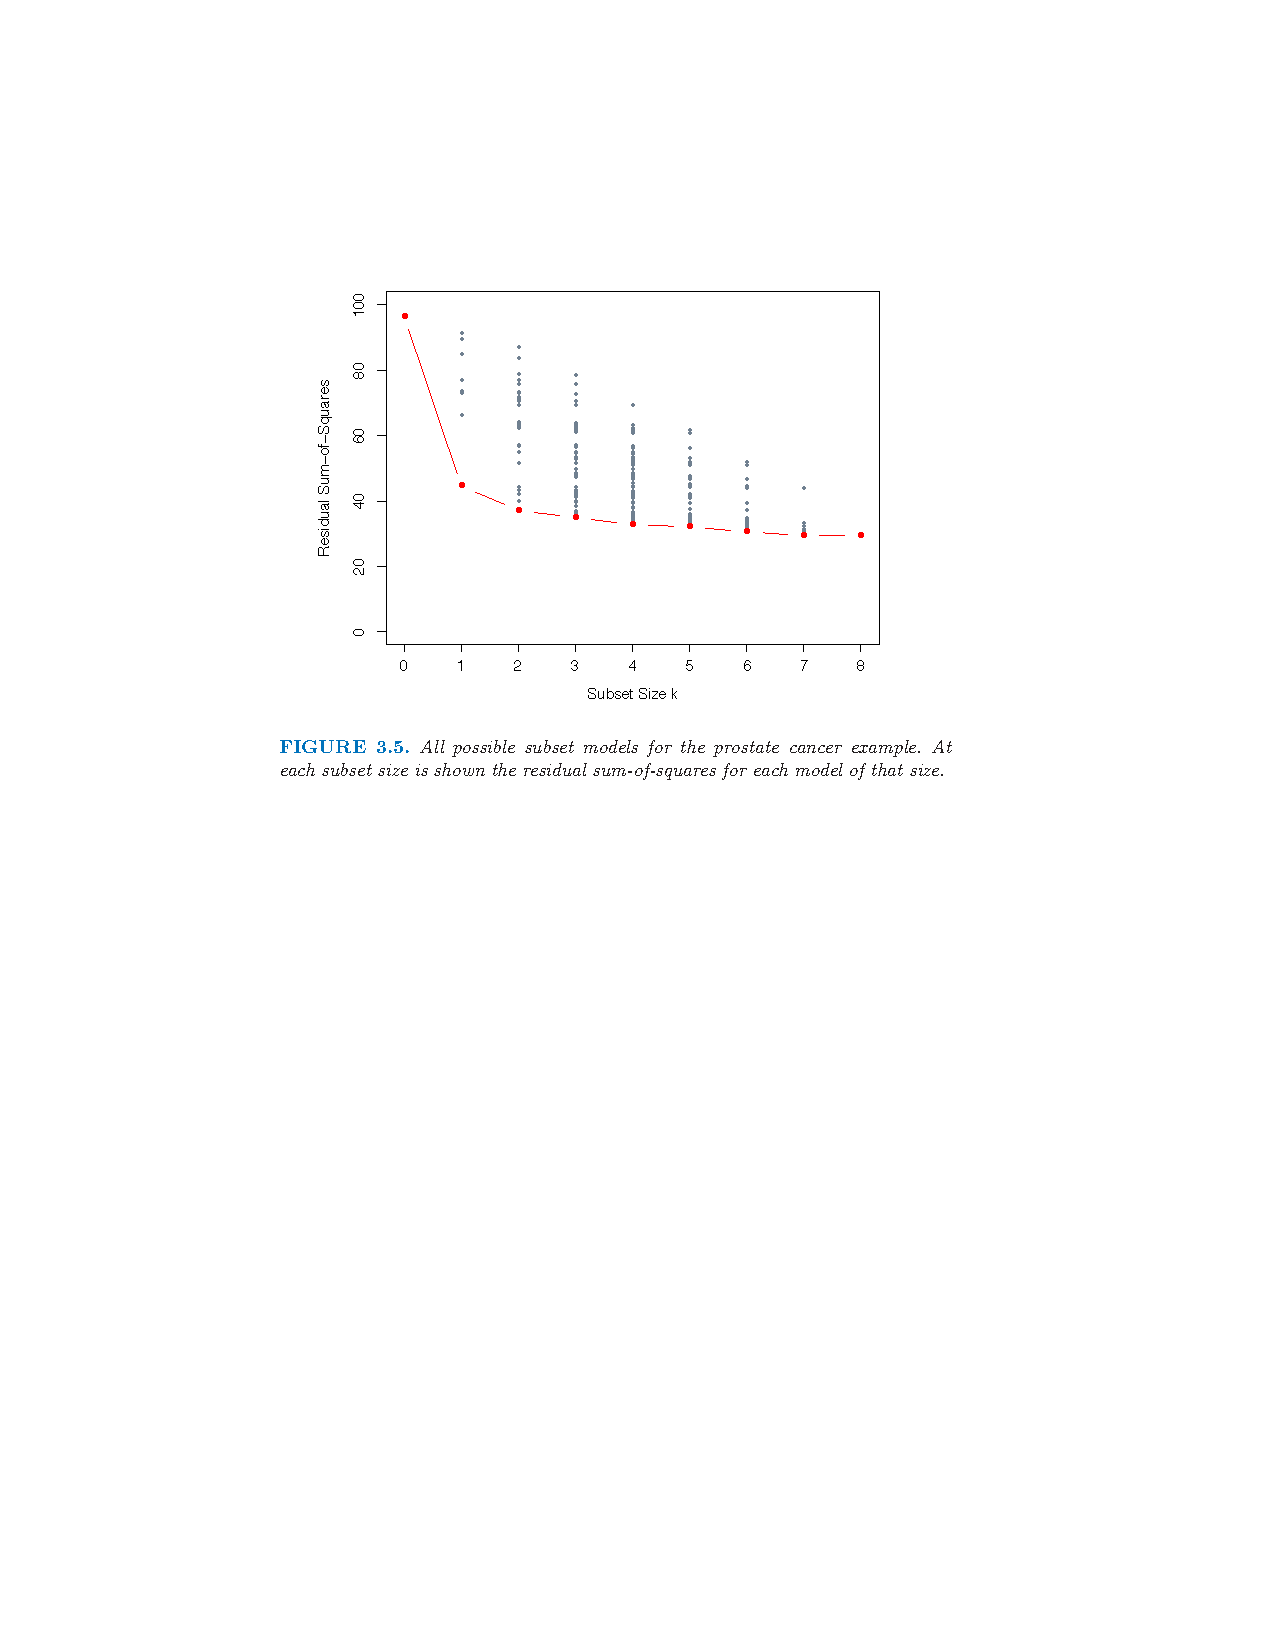
\includegraphics[height=0.9\textheight]{./resources/subsetsaic}
\end{center}
\end{frame}

\begin{frame}
\frametitle{What is orthogonality?}
\begin{itemize}
\item We can think about a world where $\langle\, x_j, x_k \rangle =0$ for $j \neq k$.
\item In this world I can get $\beta_j$ by regressing $y$ on $x_j$ by simple linear regression.
\item I could do this for each $j$ and the resulting vector $\beta$ would be the same as running multiple regression.
\item We could try and transform $X$ so that it forms an \alert{orthogonal basis}.
\item Unless we are running regressions by hand this doesn't seem tremendously helpful.
\item However, in practice this is often what your software does!
\end{itemize}
\end{frame}

\begin{frame}
\frametitle{Gram-Schmidt/QR Decomposition}
\small
\begin{enumerate}
\item Let $x_0 = z_0 = 1$
\item For $j = 1,2,\ldots p$: Regress $x_j$ on $z_0,z_1,\ldots,z_{j-1}$  to give you $\hat{\gamma_{jl}} = \langle\, z_l, x_j \rangle/\langle\, z_l, x_l \rangle$ and residual $z_j = x_j  - \sum_{k=0}^{j-1} \hat{\gamma_{kj}} z_k$.
\item With your transformed orthogonal basis $\mathbf{z}$ you can now regress $y$ on $z_p$ one by one to obtain $\hat{\beta}_p$.
\end{enumerate}
What does this do?
\begin{itemize}
\item The resulting vector $\hat{\beta}$ has been adjusted to deliver the marginal contribution of $x_j$ on $y$ after adjusting for all $x_{-j}$.
\item If $x_j$ is highly correlated with other $x_k$'s then the residual $z_j$ will be close to zero and the coefficient will be unstable.
\item This will be true for any variables $x_l$ within a set of correlated variables.
\item We can delete any one of them to resolve this issue.
\end{itemize}
\end{frame}


\begin{frame}
\frametitle{QR Decomposition (Technical Details)}
\small
QR Decomposition has a matrix form which regression software uses:
\begin{eqnarray*}
\mathbf{X} &=& \mathbf{Z \Gamma} \\
    &=& \mathbf{\underbrace{Z D^{-1}}_{Q} \underbrace{D \Gamma}_{R}} \\
    \hat{\beta} &=& \mathbf{R^{-1} Q' y}\\
    \hat{\mathbf{y}} &=& \mathbf{Q Q'} \mathbf{y}
\end{eqnarray*}
\vspace{-0.5cm}
\begin{itemize}
\item $Z$ is the matrix of the orthogonalized residuals $z_j$'s.
\item $\Gamma$ is upper triangular matrix with entries $\hat{\gamma}_{kj}$
\item $D$ is diagonal matrix with entries $|| z_j ||$.
\item $Q$ is $N \times ((p+1)$ orthogonal  matrix $Q'Q = I$ 
\item $R$ is $(p+1) \times (p+1)$ upper triangular matrix.
\end{itemize}
\end{frame}


\begin{frame}
\frametitle{What happens in practice?}
What are people likely doing in practice:
\begin{itemize}
\item Start with a single $x$ variable and then slowly add more until additional $x$'s were insignificant
\item Start with all possible $x$ variables and drop those where $t$-statistics were insignificant.
\item These procedures actually make some sense if the columns of $X$ are \alert{linearly independent} or \alert{orthogonal}.
\item In practice our regressors are often correlated (sometimes highly so).
\end{itemize}
\end{frame}


\begin{frame}
\frametitle{Forward Stepwise Regression}
Consider the following \alert{greedy algorithm}
\begin{enumerate}
\item Start with an empty model and add a constant $\overline{y}$.
\item Then run $K$ single-variable regressions, choose the $x_k$ with the highest $t$-statistic call this $x^{(1)}$.
\item Now run $K-1$ two variable regressions where the constant and $x^{(1)}$ and choose $x^{(2)}$ as regression where $x_k$ has the highest t-statistic.
\item Now run $K-2$ three variable regressions where the constant and $x^{(1)},x^{(2)}$
\item You get the idea!
\end{enumerate}
We stop when the $x_k$ with the highest t-statistic is below some threshold (often 20\% significance).
\end{frame}


\begin{frame}
\frametitle{Backwards Stepwise Regression}
\begin{enumerate}
\item Start with an full model.
\item Remove the $x$ variable with the lowest $t$-statistic. Call this $x^{(k)}$.
\item Re-run the regression without $x^{(k)}$.
\item Repeat until the smallest $t$-statistic exceeds some threshold.
\end{enumerate}
\end{frame}


\begin{frame}
\frametitle{Comparison}
\begin{itemize}
\item Backwards and fowards stepwise regression tend to give similar choices (but not always).
\item Everything is trivial if $X$'s columns are orthogonal (computer has some tricks otherwise- $QR$).
\item Forward stepwise works when we have more regressors than observations $K > N$.
\item I proposed the $t$-stat here but some packages use AIC/BIC as the criteria.
\item We should also be careful to \alert{group dummy variables together} as a single regressor.
\item These are implemented in \texttt{step} in R and \texttt{stepwise} in Stata.
\item We probably want to adjust our standard errors for the fact that we have run many regressions in sequence before arriving at our model. \alert{In practice not enough people do this!}
\end{itemize}
\end{frame}


\begin{frame}
\frametitle{(Incremental) Forward Stagewise Regression}
As an alternative consider:
\begin{enumerate}
\item Start with $r= y$ and $(\beta_1, \ldots, \beta_p) = 0$.
\item Find the predictor $x_j$ most correlated with $r$.
\item Update $\beta_j \leftarrow \beta_j + \delta_j$ where $\delta_j = \epsilon \cdot sgn \langle r , x_j \rangle$.
\item Update $r \leftarrow r - \delta_j \cdot x_j$ and repeat for $S$ steps.
\end{enumerate}
\begin{itemize}
\item Alternative $\delta_j =  \langle r , x_j \rangle$
\item We can continue until no regressors have correlation with residuals 
\item This is very slow (it takes many many $S$).
\item Sometimes slowness can be good -- in high dimensions to avoid overfitting.
\end{itemize}
\end{frame}



\begin{frame}
\frametitle{Stepwise selection proedures}
\begin{center}
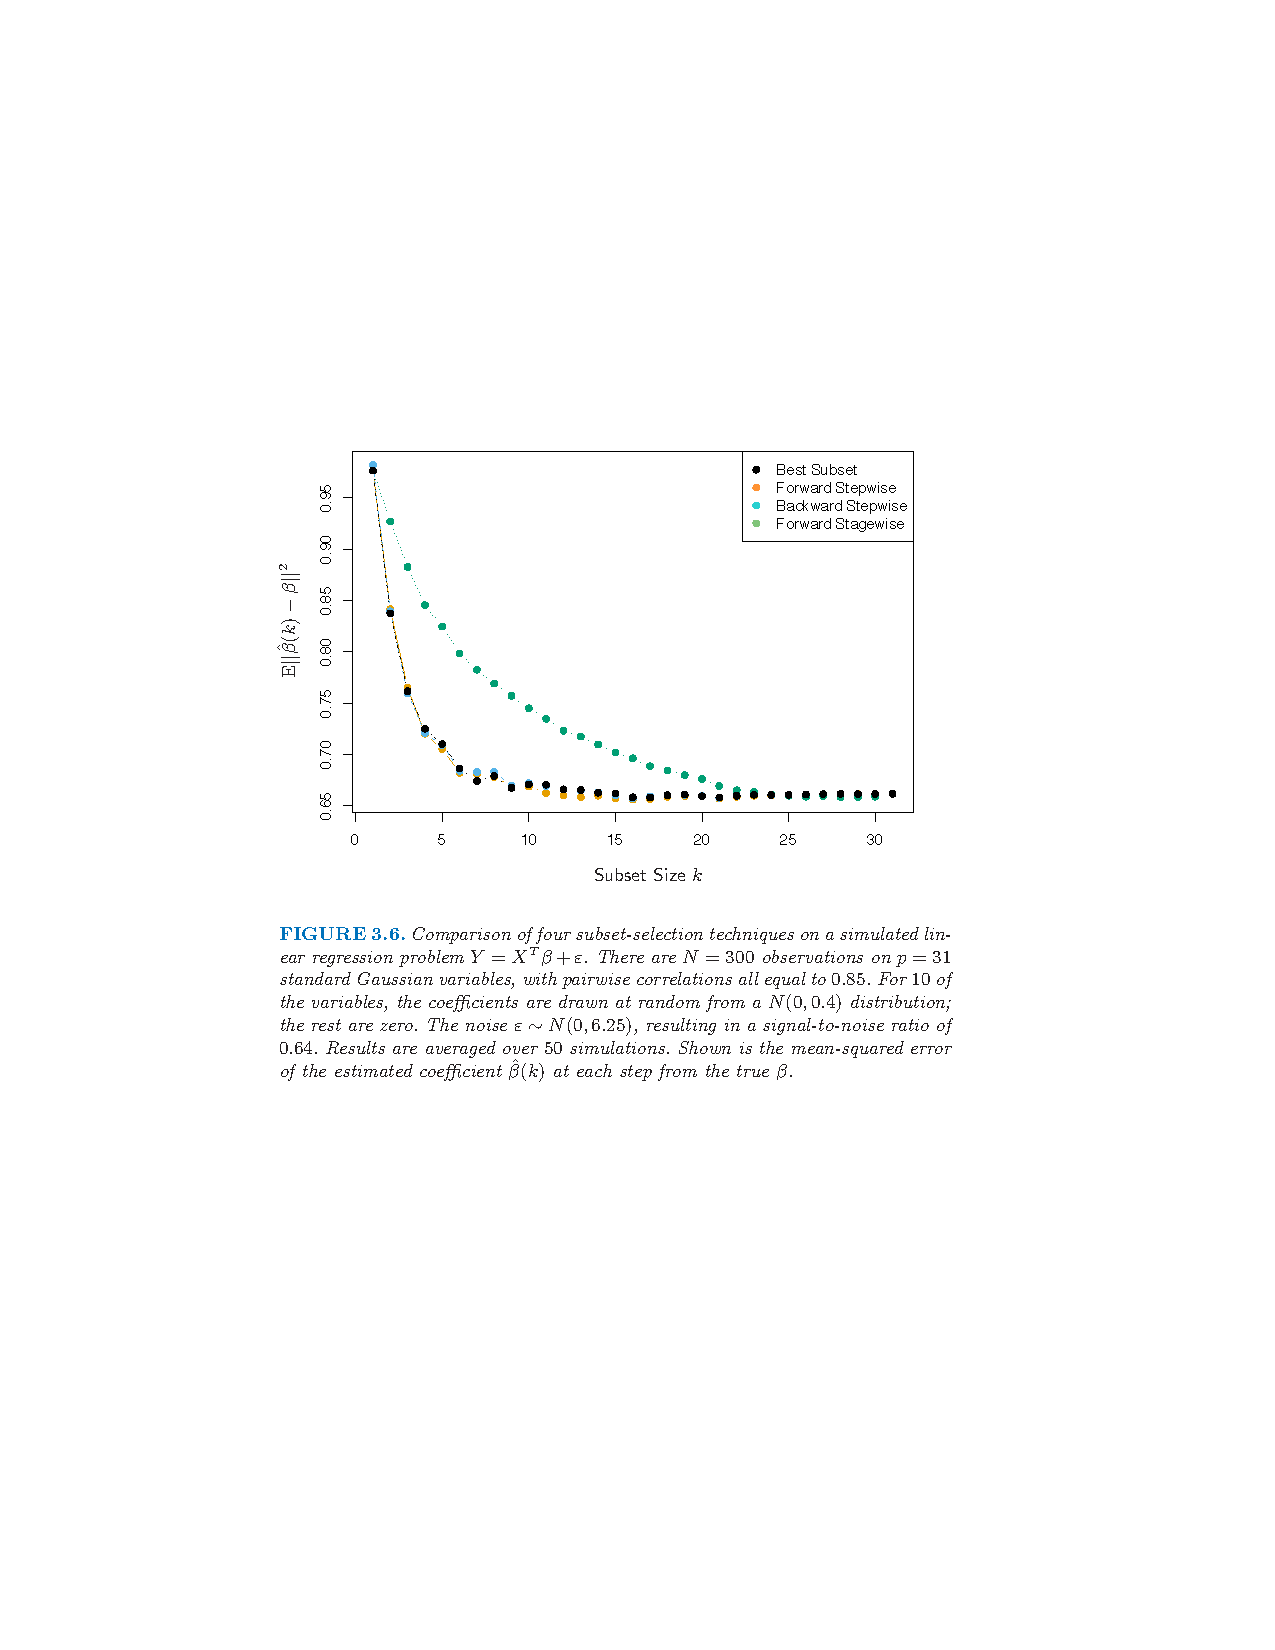
\includegraphics[height=0.9\textheight]{./resources/subsetstepwise}
\end{center}
\end{frame}




\begin{frame}
\frametitle{Multiple Testing Problem}
\begin{itemize}
\item A big deal in Econometrics frequently ignored in applied work is the \alert{Multiple Testing Problem}
\item You didn't just pick the regression in your table and run that without considering any others.
\item This means that your $t$ and $F$ stats are going to be too large!! (Standard errors too small!)
\item How much bigger should they be?
\begin{itemize}
\item Analytic size corrections can be tricky and data dependent
\item Bootstrap/Monte-Carlo studies should give you a better idea.
\end{itemize}
\end{itemize}
\end{frame}




\end{document}
